\section{Auswertung der Konzepte und Auswahl eines Konzepts}
Die entwickelten Konzepte wurden in nachfolgender Tabelle \ref{fig:TabEvalTwo} nach den VDI-Richtlinien \textit{2222} und \textit{2225} bewertet. Hierf\"{u}r wurden die Konzeptvarianten mit den Mindest-, Ziel- und Wunschanforderungen aus der Anforderungsliste verglichen und den Punkte von eins bis vier zugeordnet. Unterschieden wurde zwischen technischen und wirtschaftlichen Bewertungsmerkmalen. Da jede Anforderung eine unterschiedliche Relevanz besitzt, wurden zus\"{a}tzlich die Gewichtungsfaktoren ebenfalls von eins bis vier eingef\"{u}hrt.
\\\\
Die Bewertungspunktzahl von jeder Anforderung wurde mit der zugeh\"{o}rigen Gewichtung summiert und anschlie{\ss}end wurden alle Bewertungen aufsummiert. Dieses Verfahren wird an jedem Konzept angewandt, sodass am Ende die Gesamtpunktzahl von jedem Konzept errechnet ist. In diesem Fall gab es f\"{u}nf Konzeptvarianten und somit auch f\"{u}nf Gesamtpunktzahlen auszuwerten.
\\\\
Anders als in der VDI-Richtlinie wurde die wirtschaftliche Wertigkeit nach dem gleichen Verfahren wie die technische Wertigkeit bewertet. Die wirtschaftliche Wertigkeit in den VDI-Richtlinien wird durch die Herstellungskosten bestimmt, welche zus\"{a}tzlich die Ermittlung der Materialkosten nach VDI \textit{2225} erfordert. In dieser Arbeit wird auf dieses Vorgehen verzichtet, da das Hauptaugenmerk auf der technischen Bewertung liegt. Die Kosten wurden als wirtschaftliche Anforderung nicht vernachl\"{a}ssigt, jedoch nur anhand der Herstellerinformationen \"{u}berschlagen. Die Wertigkeit wurde mit folgender Gleichung berechnet
\begin{align*}
	x_g = \frac{g_1p_1 + g_2p_2 + ... + g_np_n}{(g_1 + g_2 + ... + g_n)p_\textit{max}}
\end{align*}
Die Ergebnisse der Wertigkeiten f\"{u}r die Konzeptvarianten eins bist f\"{u}nf sind der Tabelle x zu entnehmen. F\"{u}r eine graphische Darstellung der Ergebnisse wurden die technische Wertigkeit als \(x\)-Koordinate und die wirtschaftliche Wertigkeit als \(y\)-Koordinate in ein sogenanntes \textit{s-Diagramm} eingetragen. Der Punkt mit den Koordinaten \(x\) und \(y\) wird als St\"{a}rke der Konzeptvariante bezeichnet. Die Ideall\"{o}sung \(s_i\) mit den Werte \(x = 1\) und \(y = 1\) wurde auch in das Diagramm eingetragen und mit einer Geraden mit dem Ursprung verbunden. Die Wertigkeit, mit der h\"{o}chsten St\"{a}rke, hat auch die h\"{o}chste technisch-wirtschaftliche Bewertung erhalten, welche in dieser Bewertung die Konzeptvariante vier ist.
\begin{figure}[H]
        \myfloatalign
        {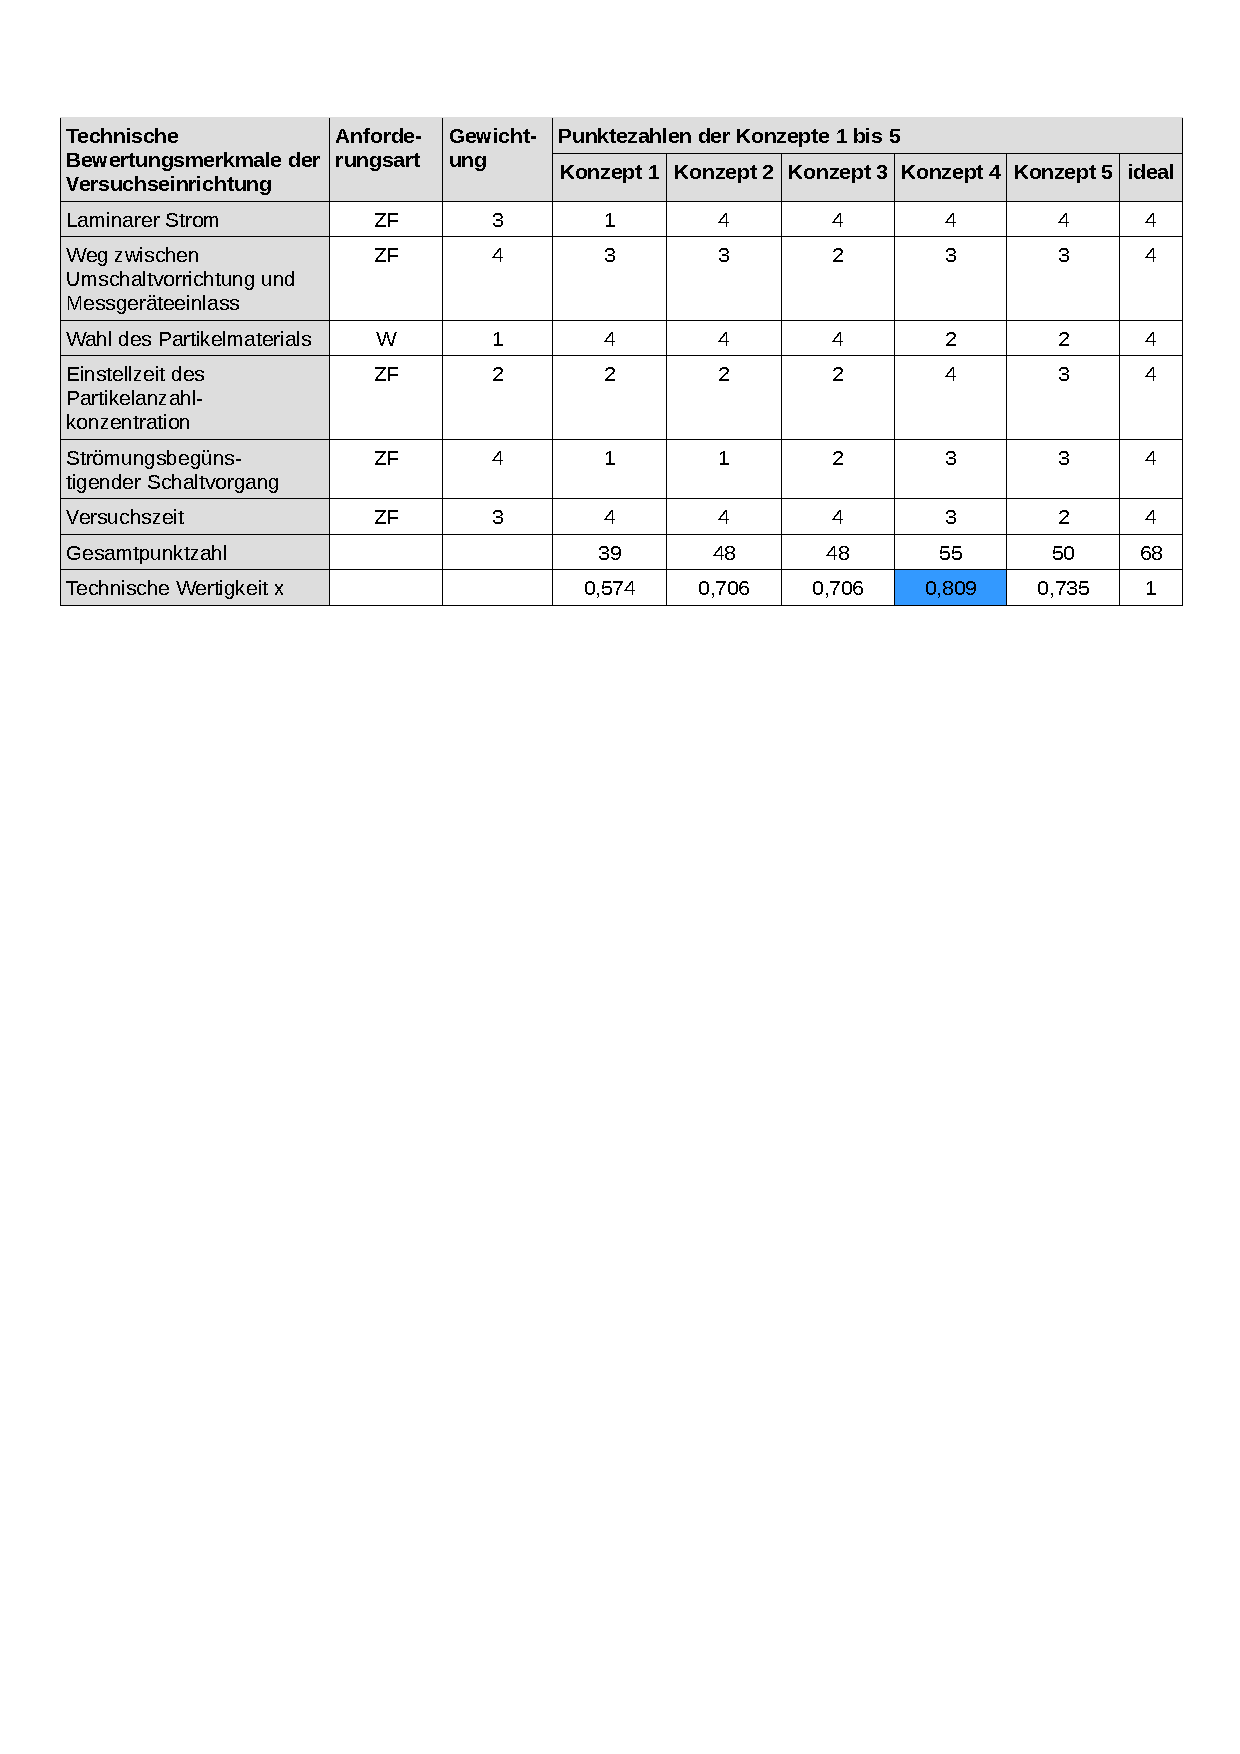
\includegraphics[width=.8\linewidth]{gfx/conclusion/TabEvalTwo.pdf}} \quad
        \caption[Technische Bewertung der Konzepte]
        {Technische Bewertung der Konzepte}
        \label{fig:TabEvalOne}
\end{figure}
\begin{figure}[H]
        \myfloatalign
        {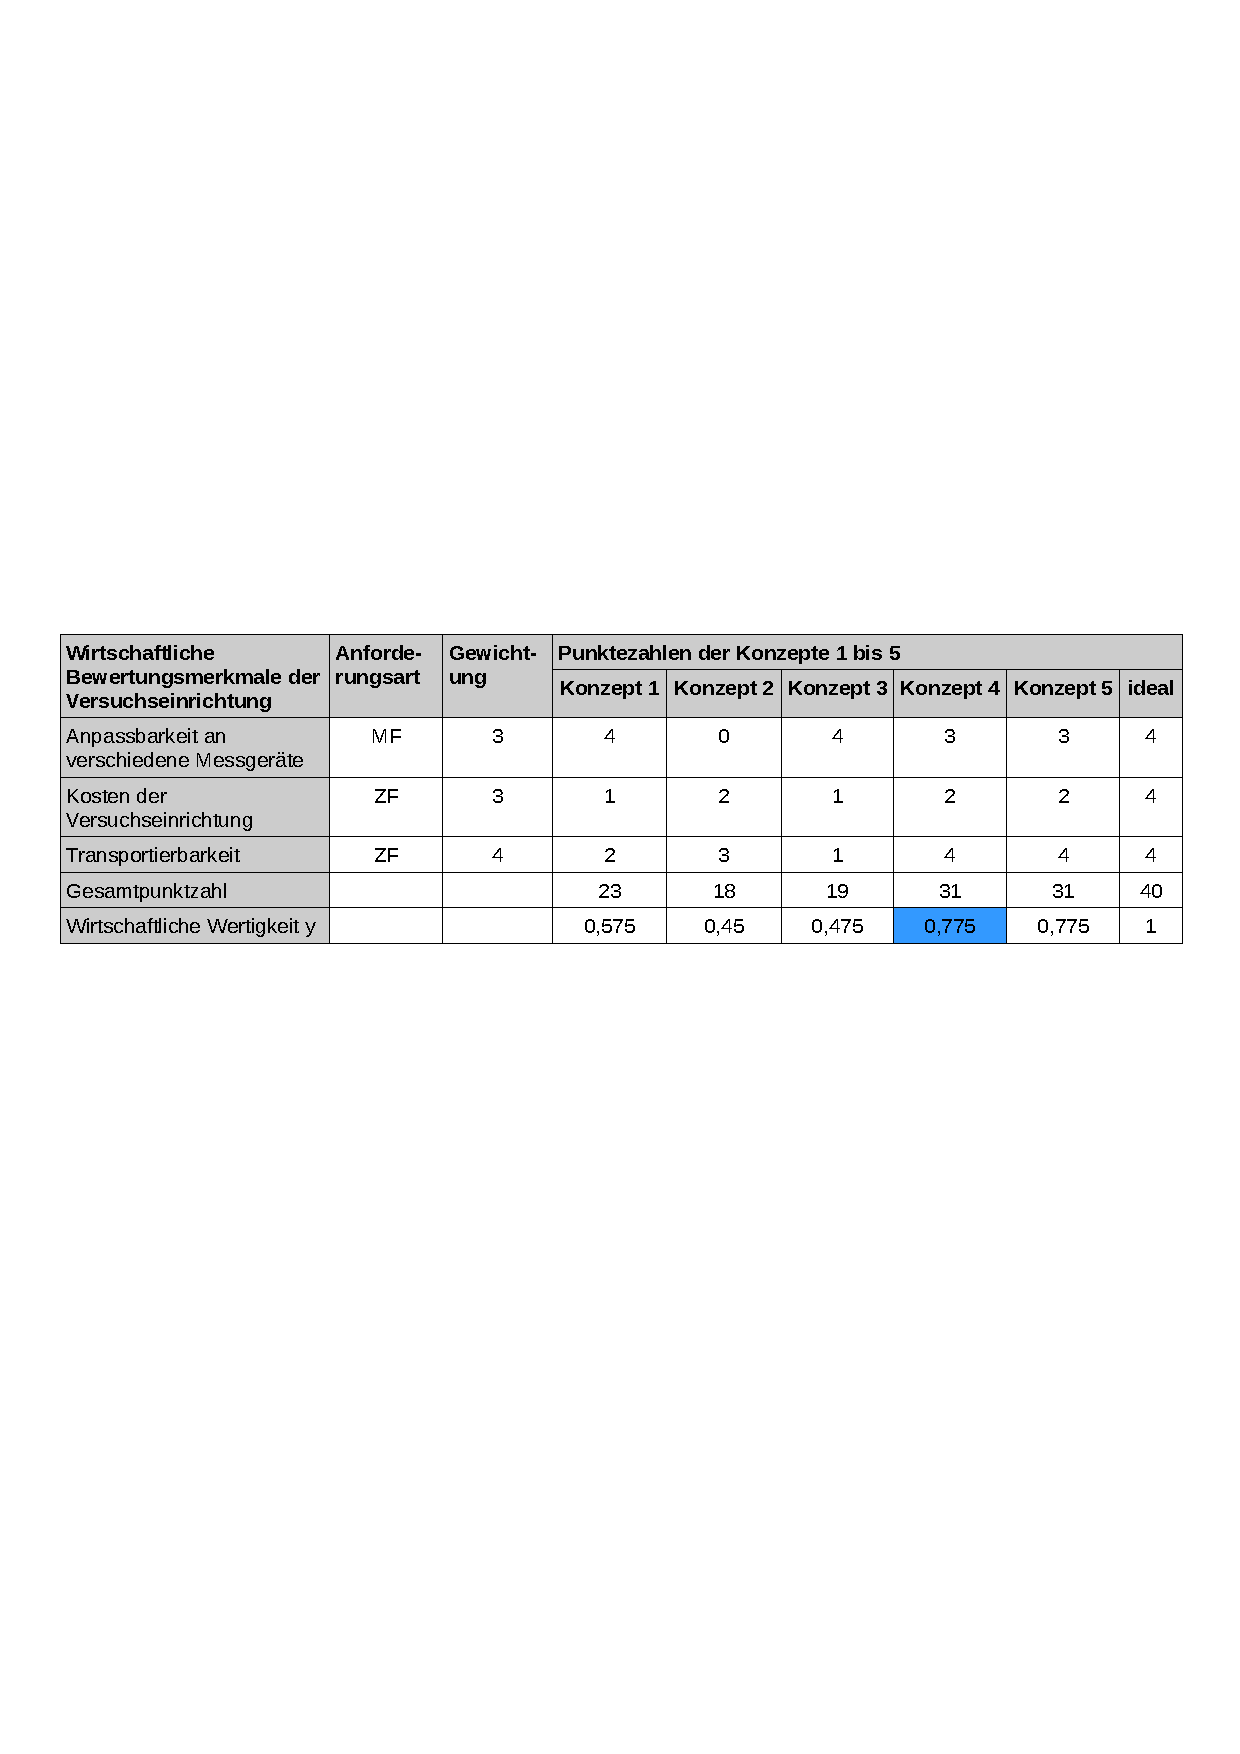
\includegraphics[width=.8\linewidth]{gfx/conclusion/TabEvalThree.pdf}} \quad
        \caption[Wirtschaftliche Bewertung der Konzepte]
        {Wirtschaftliche Bewertung der Konzepte}
        \label{fig:TabEvalOne}
\end{figure}
\begin{figure}[H]
        \myfloatalign
        {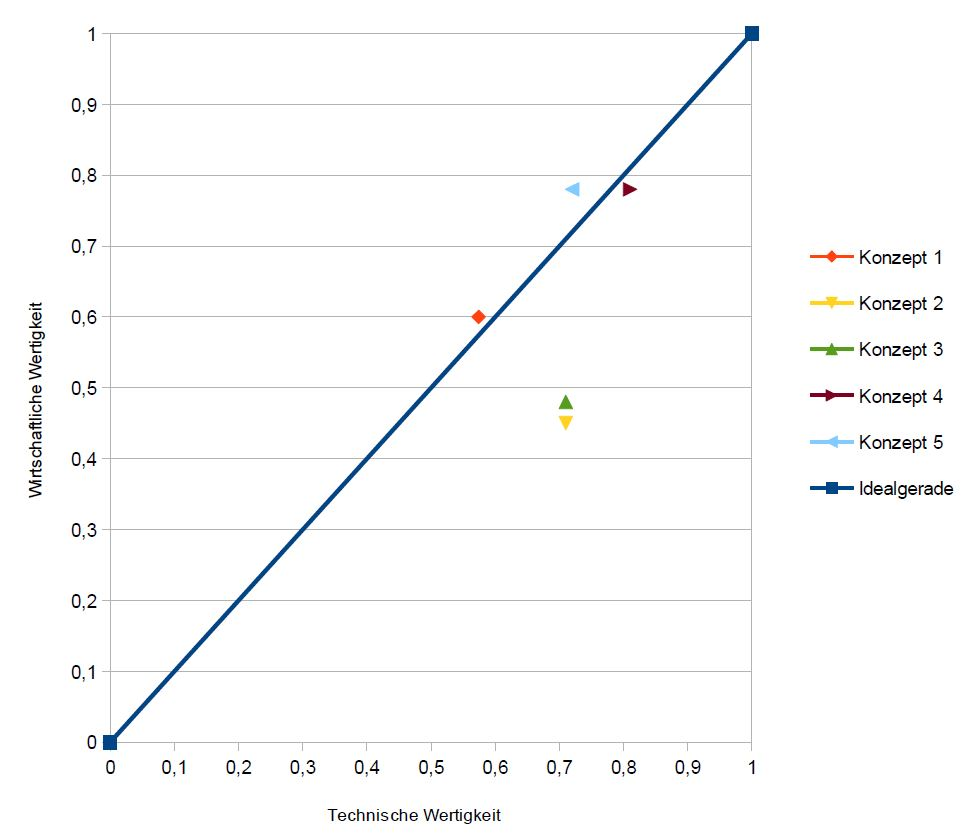
\includegraphics[width=.6\linewidth]{gfx/conclusion/s_diagram.jpg}} \quad
        \caption[Auswertung der Konzeptbewertung - Konzept 4 hat den kleinsten Abstand zum Idealwert]
        {Auswertung der Konzeptbewertung - Konzept 4 hat den kleinsten Abstand zum Idealwert}
        \label{fig:TabEvalOne}
\end{figure}